\documentclass{article}

\usepackage{amsmath}
\usepackage{graphicx}
\usepackage{subfig}

\title{Umbrella Sampling + WHAM}
\author{Henry Bloom, Arnav Brahmasandra}
\date{\today}

\begin{document}

\maketitle

\section{Motivation}
Molecular systems often exhibit high free energy barriers that impede adequate sampling of configurational space in standard simulations. 
Umbrella sampling addresses this by introducing biasing potentials to enhance sampling in targeted regions, stitching the biased distributions together using WHAM.
WHAM provides a systematic framework to reconstruct unbiased free energy profiles from biased simulations. 

\section{Theory}

\subsection{Umbrella Sampling}
Consider some system with a potential $U(r^N)$. 
Traditional sampling methods may suffer from poor ergodicity due to certain energy landscapes, particularly if the confifuration space has many high-energy barriers that may trap the trajectory in a local minimum.
Introduced by Torrie and Valleau in 1977, umbrella sampling uses bias potentials to encourage sampling of potentially inaccessible states.
The biased distributions are then used to reconstruct an unbiased distribution and calculate quantities of interest, such as the free energy of the system.

\subsubsection{Reaction Coordinate}
We will introduce the notion of a reaction coordinate $q = f(r^N)$, an abstract one-dimensional parameter that unambiguously measures progress along a reaction pathway or transition between states.
Some examples of a reaction coordinate, both geometric and non-geometric, include bond distance, bond angle, torsion, dihedral angle, bond order, Hydrogen bonds, and RMSD. 
The free energy of a system is often considered as a function of reaction coordinate to demonstrate in some schematic form the potential energy profile associated to the reaction.

\subsubsection{Bias Potentials}
Umbrella sampling introduces a window-specific soft restraint biasing potential $W_i(q, s)$, such that the total potential for window $i$ becomes $U_i^\text{biased}(r^N) = U(r^N) + W_i(f(r^N))$.
Often, the restraint is chosen to be a harmonic potential of the form $W_i(f(r^N),s) = \frac{1}{2} \kappa (f(r^N) - s_i)^2$ centered around a chosen $s_i$.

\subsubsection{Simulations}
In umbrella sampling, run a series of $n$ simulations with different biasing potentials, collecting a biased distribution of values of $q$.
Essentially, each simulation can be thought of as generating a histogram of values of $q$ primarily located within a "window" corresponding to the bias potential chosen.
The aim following the computation of these biased distributions is to first unbias them, and then to use the unbiased distributions to calculate the free energy of the system.

\subsection{WHAM}
The weighted histogram analysis method (WHAM) is the method for unbiasing the biased distributions that is used in conjunction with umbrella sampling.

\subsubsection{Unbiasing the Probabilities}
We begin with biased probabilities:
$$\tilde{P}(q, s_k) = e^{\beta A_k} \int d^N r^N e^{-\beta U(r^N)} e^{- \beta W(f(r^N), s^{(k)})}\delta(f(r^N) - q)$$
We can then express the free energy due to each individual restraining potential, $A_k$, as follows:
$$e^{-\beta A_k} = \int d^N r^N e^{-\beta U(r^N)} e^{-\beta W(f(r^N), s^{(k)})} = e^{-\beta A_0} \left \langle e^{- \beta W(f(r^N), s^{(k)})} \right \rangle$$
Note the following:
$$e^{-\beta A_0} = \int d^N r^N e^{-\beta U(r^N)} = Z$$
We can use this process to calculate the unbiased potential from the $k$-th window as follows:
$$ P_k(q) = e^{-\beta(A_k - A_0)} e^{\beta W\left(q, s^{(k)}\right)} \tilde{P}(q, s^{(k)}) $$

\subsubsection{Reconstructing the Global Distribution}
Our aim is to use the $k$ unbiased distribution estimates from the simulations to construct the global distribution $P(q)$ while minimizing statistical error.
We can set this up as follows:
\begin{align*}
    P(q) = &\sum_{k=1}^n C_k(q) P_k(q)\\
    \text{subject to} &\sum_{k=1}^n C_k(q) = 1
\end{align*}
The aim is to optimize the statistical error of $P(q)$ while satisfying the given constriant.

\subsubsection{Statistical Error}
We first aim to express the statistical error of each biased distribution using its corresponding histogram by the following:
$$ \tilde{P}(q, s^{(k)}) \approx \frac{1}{n_k \Delta q} \tilde{H}_k(q) $$
Where $\tilde{H}_k$ is the histogram from the $k$-th simulation, $n_k$ is the number of configurations sampled, and $\Delta q$ is the bin width.
The statistical error in this distribution is then expressed as follows:
$$ \tilde{\sigma}_k^2 = \epsilon_k(q) \frac{1}{n_k \Delta q} \tilde{H}_k(q)$$
Where $\epsilon_k(q)$ is the error of the sample with respect to the actual biased distribution.
\\\\
We can propogate this error to estimate the error in the $k$-th unbiased distribution:
\begin{align*}
    P_k(q) &= e^{-\beta(A_k - A_0)} e^{\beta W\left(q, s^{(k)}\right)} \tilde{P}(q, s^{(k)})\\
    \sigma_k^2 &= e^{-2 \beta (A_k - A_0)}e^{2 \beta W(q, s^{(k)})}\tilde{\sigma}_k^2
\end{align*}
Thus, the total statistical error in the global distribution will be:
$$ \sigma^2 = \sum_{k=1}^n C_k^2(q) \sigma_k^2 $$

\subsection{Minimizing the Statistical Error}
We can use Lagrange multipliers to perform this constrained minimization by instead minimizing the following:
$$ \Sigma^2 = \sum_{k=1}^n C_k^2(q) \sigma_k^2 - \lambda \left(\sum_{k=1}^n C_k(q) - 1\right)$$

% Before calculating, we will make the simplifying assumptions that $\epsilon_k(q)$ is constant for all $k$ and that the biased histograms $\tilde{H_k}(q)$ are proportionate to a direct biasing of the unbiased global $P(q)$: $\tilde{H_k}(q) \propto e^{\beta (A_k - A_0)} * e^{-\beta W(q, s^{(k)})} * P(q)$.
% We can now set $\frac{\partial \Sigma^2}{\partial C_k(q)} = 0$ and solve:
% \begin{align*}
%     0 &= \frac{\partial \Sigma^2}{\partial C_k(q)}\\
%     &= \frac{\partial}{\partial C_k(q)} \left[\sum_{k=1}^n C_k^2(q) \sigma_k^2 - \lambda \left(\sum_{k=1}^n C_k(q) - 1\right)\right]\\
%     &= \frac{\partial}{\partial C_k(q)} \left[\sum_{k=1}^n C_k^2(q) \left(e^{-2 \beta (A_k - A_0)}e^{2 \beta W(q, s^{(k)})}\tilde{\sigma}_k^2\right)- \lambda \left(\sum_{k=1}^n C_k(q) - 1\right) \right]\\
%     &= \frac{\partial}{\partial C_k(q)} \left[\sum_{k=1}^n C_k^2(q) \left(e^{-2 \beta (A_k - A_0)}e^{2 \beta W(q, s^{(k)})} \epsilon_k(q) \frac{1}{n_k \Delta q} \tilde{H}_k(q) \right)- \lambda \left(\sum_{k=1}^n C_k(q) - 1\right) \right]\\
%     &= \frac{\partial}{\partial C_k(q)} \left[\sum_{k=1}^n C_k^2(q) \left(e^{-2 \beta (A_k - A_0)}e^{2 \beta W(q, s^{(k)})} \epsilon(q) \frac{1}{n_k \Delta q} \tilde{H}_k(q) \right)- \lambda \left(\sum_{k=1}^n C_k(q) - 1\right) \right]\\
% \end{align*}

After solving for $\lambda$ and $C_k(q)$ for all $k$ by setting $\frac{\partial \Sigma^2}{\partial C_k(q)} = 0$, we make the simplifying assumptions that $\epsilon_k(q)$ is constant for all $k$ and that the biased histograms $\tilde{H_k}(q)$ are proportionate to a direct biasing of the unbiased global $P(q)$: $\tilde{H_k}(q) \propto e^{\beta (A_k - A_0)} * e^{-\beta W(q, s^{(k)})} * P(q)$.
Finally, plugging the $C_k(q)$ coefficients back into the equation for $P(q)$ provides us with a set of equations to solve iteratively:

\begin{align*}
    P(q) &= \frac{\sum_{k=1}^n n_k \tilde{P_k}(q)}{\sum_{k=1}^n n_k e^{\beta (A_k - A_0)} e^{-\beta W(q, s^{(k)})}}\\
    e^{\beta (A_k - A_0)} &= \int \text{d}q P(q) e^{-\beta W(q, s^{(k)})}
\end{align*}

Following the iterative solving of these equations, we can obtain the free energy from $P(q)$ through the following formula:
$$ A(q) = -\frac{1}{\beta} \ln P(q) + A_0 $$


\section{Systems}
In this project, we apply umbrella sampling and WHAM to three main systems: a one-dimensional two-welled potential, a one-dimensional multi-welled potential, and a two-dimensional Muller-Brown potential. These energy landscapes are chosen to demonstrate the effectiveness of umbrella sampling and WHAM, when applied to systems with energy barriers that impede adequate sampling of configurational space in standard simulations. In all of these systems, we consider the only \textit{one} particle in the system, and the reaction coordinate is the position of this particle. Additionally, we consider the system to be in thermal equilibrium at a temperature of $T = 50K$, to demonstrate the effectiveness of the methods in sampling the potential energy surface at a low temperature.

\subsection{1D Two-Welled Potential}

We first consider a simple one-dimensional two-welled potential of the form:

$$
V(x) = 5(x-1)^8 - \epsilon_0 e^{-\frac{\epsilon_0(x-0.5)^2}{\sigma^2}} + \epsilon_1 e^{-\frac{\epsilon_1(x-1.0)^2}{\sigma^2}} - \epsilon_2 e^{-\frac{\epsilon_2(x-1.5)^2}{\sigma^2}}
$$

\begin{figure}%
    \centering
    \subfloat[\centering Two-Welled Potential]{{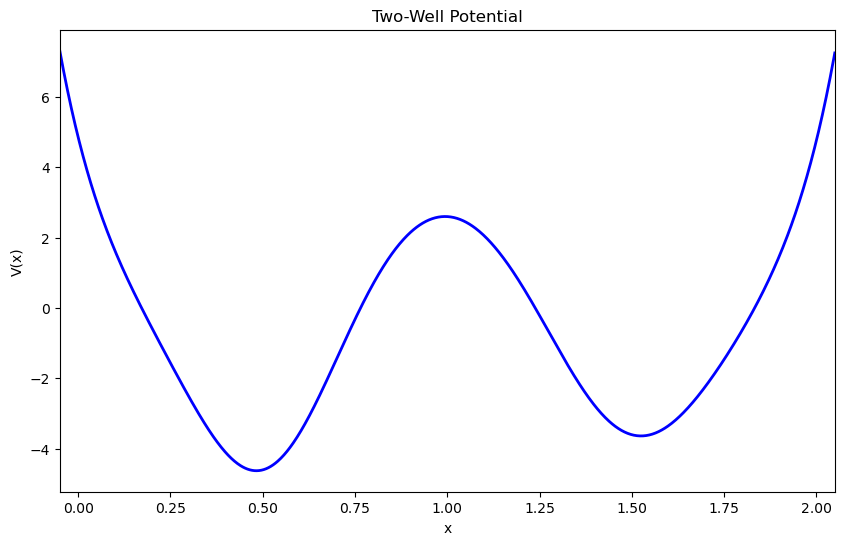
\includegraphics[width=0.46\textwidth]{images/two_well_V.png} }}%
    \qquad
    \subfloat[\centering Multi-Welled Potential]{{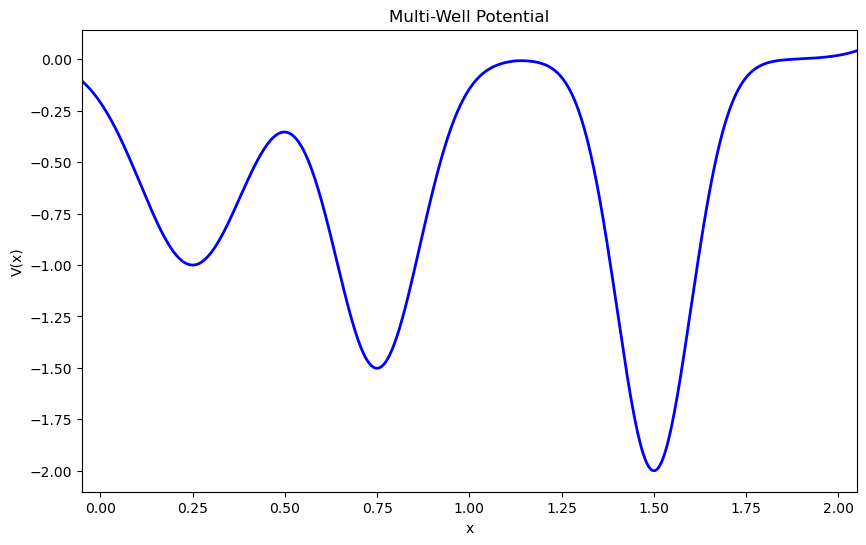
\includegraphics[width=0.46\textwidth]{images/multi_well_V.png} }}%
    \caption{1D Potentials}%
    \label{fig:1D_pots}%
\end{figure}

Where $\epsilon_0 = 5$, $\epsilon_1 = 3$, $\epsilon_2 = 4$, and $\sigma = 0.6$.

This potential has two wells at $x = 0.5$ and $x = 1.5$, and a barrier at $x = 1.0$ as seen in Figure \ref{fig:1D_pots}

\subsection{1D Multi-Welled Potential}

We then consider a one-dimensional multi-welled potential of the form:

\begin{align*}
    V(x) = 5 \min_{i} \left((x - x_i)^8\right) - \sum_  {i=1}^{3} \epsilon_i e^{-\frac{\epsilon_i(x-x_i)^2}{\sigma^2}}
\end{align*}

Where $x_1 = 0.25$, $x_2 = 0.75$, $x_3 = 1.5$, $\epsilon_0 = 1.0$, $\epsilon_1 = 1.5$, $\epsilon_2 = 2.0$, and $\sigma = 0.2$.

This potential has three wells at $x = 0.25$, $x = 0.75$, and $x = 1.5$, as seen in Figure \ref{fig:1D_pots}.

\subsection{2D Muller-Brown Potential}

Finally, we consider the two-dimensional Muller-Brown potential, which is a model potential energy surface that is often used to test optimization algorithms. The potential is given by:

\begin{align*}
    V(x, y) = \sum_{i=1}^{4} A_i e^{a_i(x - x_i)^2 + b_i(x - x_i)(y - y_i) + c_i(y - y_i)^2}
\end{align*}

Where $A_1 = -200$, $A_2 = -100$, $A_3 = -170$, $A_4 = 15$, $a_1 = -1$, $a_2 = -1$, $a_3 = -6.5$, $a_4 = 0.7$, $b_1 = 0$, $b_2 = 0$, $b_3 = 11$, $b_4 = 0.6$, $c_1 = -10$, $c_2 = -10$, $c_3 = -6.5$, $c_4 = 0.7$, $x_1 = 1$, $x_2 = 0$, $x_3 = -0.5$, $x_4 = -1$, $y_1 = 0$, $y_2 = 0.5$, $y_3 = 1.5$, $y_4 = 1$.

\begin{figure}%
    \centering
    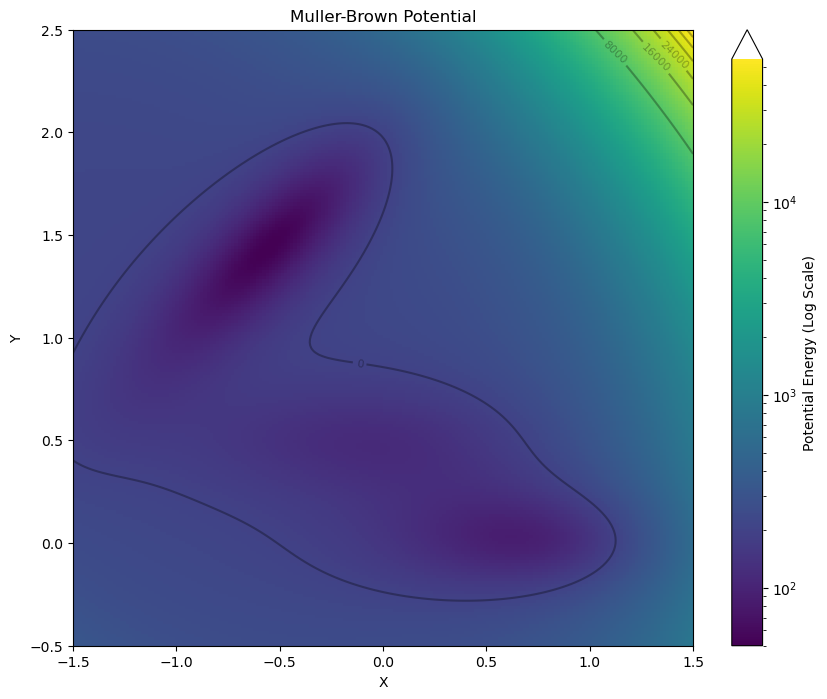
\includegraphics[width=0.6\textwidth]{images/muller_brown_V.png}
    \caption{2D Potential}%
    \label{fig:2D_pot}%
\end{figure}

This potential has three minima and two saddle points, as seen in Figure \ref{fig:2D_pot}, and is often used for testinmg algorithms that explore transition states and barriers. 

\section{Results}

\subsection{1D Two-Welled Potential}

We divided our one-dimensional two-welled potential into 100 windows, each with a biasing potential of the form $W(x, s) = \frac{1}{2} \kappa (x - s)^2$ with $\kappa = 2000$, where $s$ is the center of the window. We then ran MCMC simulations in each window, obtaining 100,000 samples for each window, resulting in biased distributions of $x$.


\subsubsection{Sampling}

\begin{figure}%
    \centering
    \subfloat[\centering Trace Plot]{{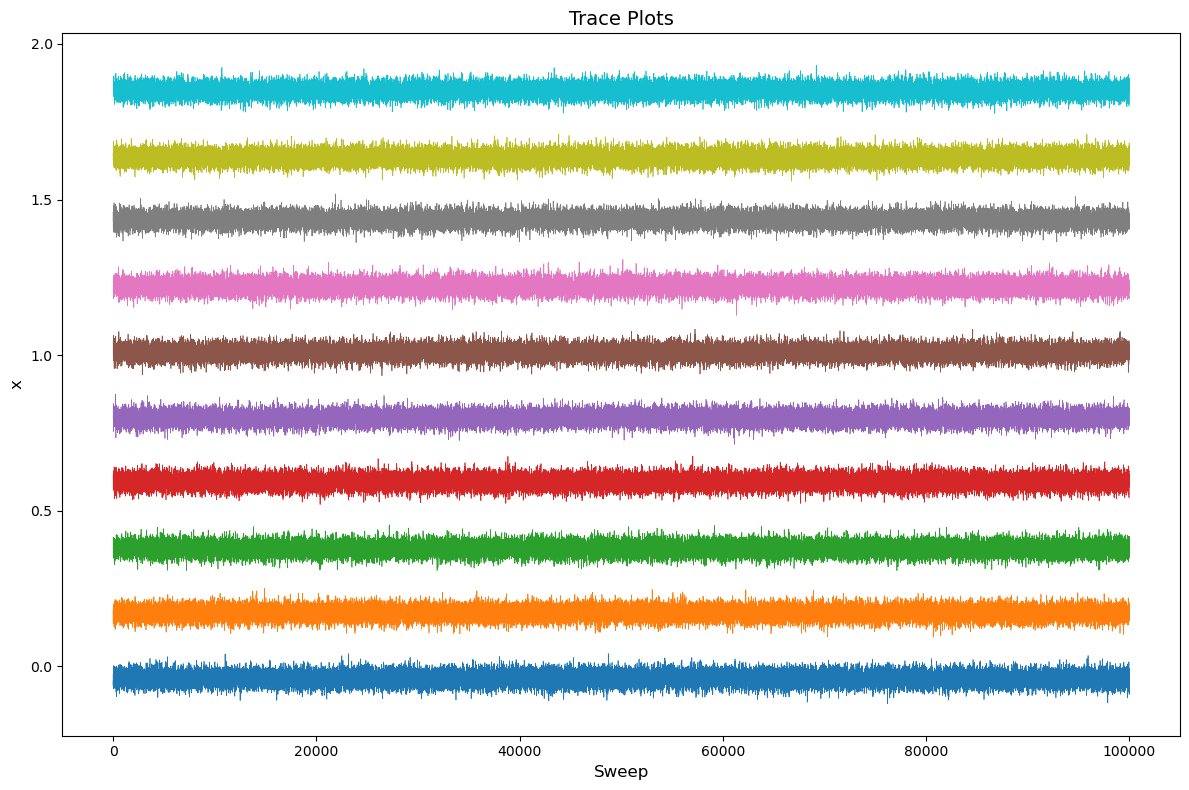
\includegraphics[width=0.46\textwidth]{images/two_well_V_trace_plot.png} }}%
    \qquad
    \subfloat[\centering Sampled Densities]{{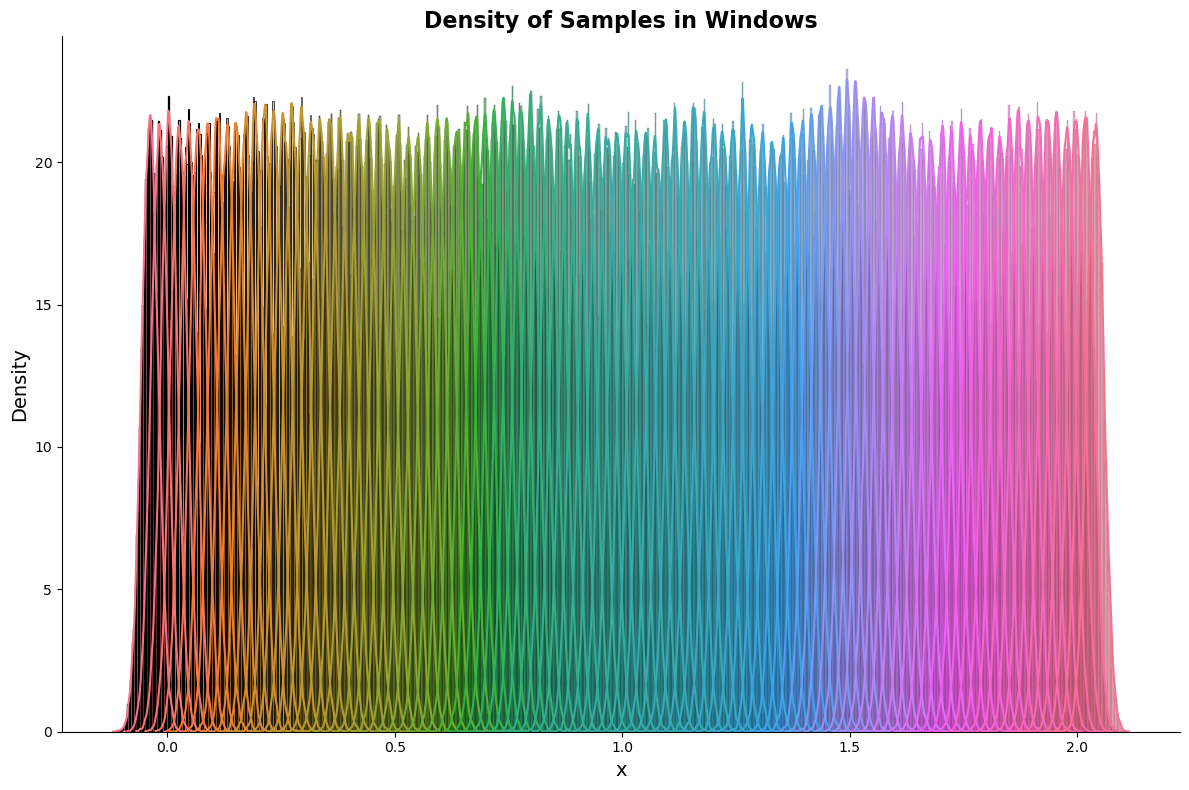
\includegraphics[width=0.46\textwidth]{images/two_well_window_sample_dens.png} }}%
    \caption{Confirmation of Window Sampling Success}%
    \label{fig:converge_diag}%
\end{figure}

% \begin{figure}%
%     \centering
%     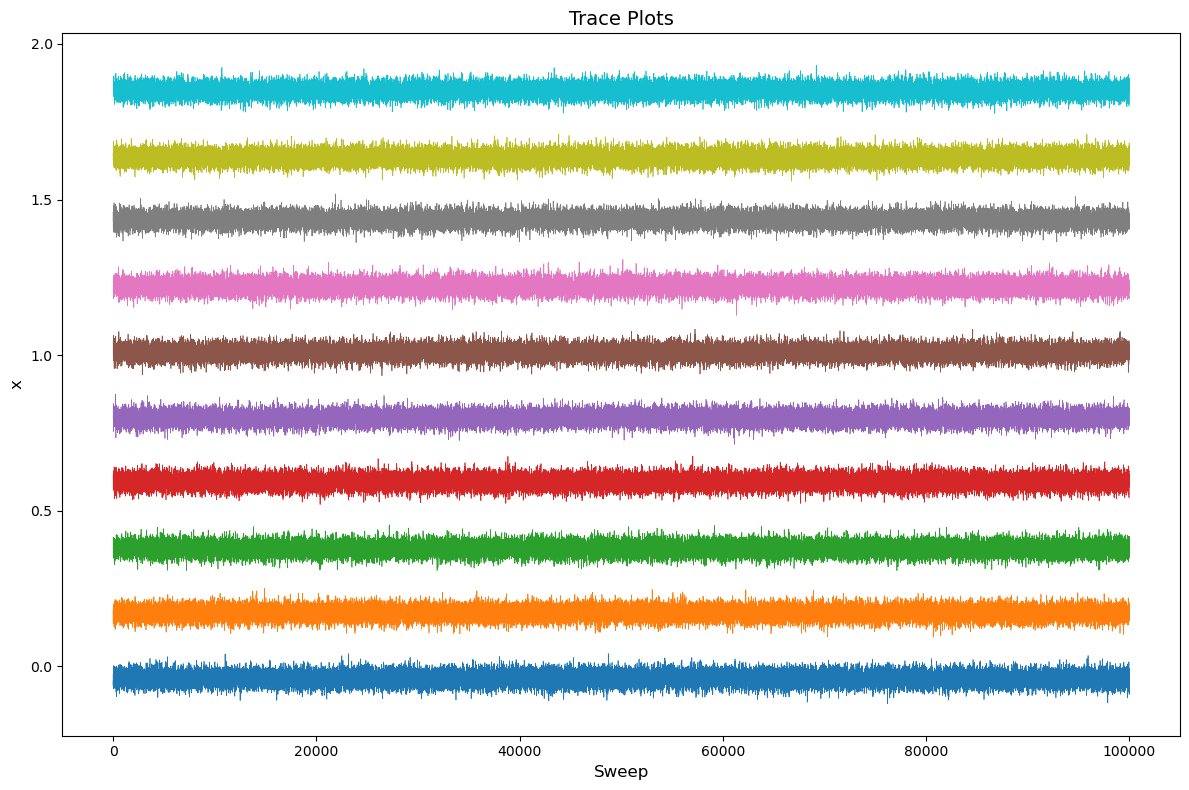
\includegraphics[width=0.6\textwidth]{images/two_well_V_trace_plot.png}
%     \caption{Trace Plot}%
%     \label{fig:trace_plot_two_well}%
% \end{figure}

In Figure \ref{fig:converge_diag}, we plot the trace plot of the biased distributions of $x$ for 10 windows. We can see that the samples are stable and oscillate around the center of the window, indicating that the biasing potential has effectively encouraged sampling in the regions of the potential that would otherwise be difficult to sample. This gives us confirmation that the biasing potential is working as intended.

Additionally, we plot the sampled densities of $x$ for all the windows in Figure \ref{fig:converge_diag}. We can see that the sampling results in a relatively flat distribution, indicating that the biasing potential has effectively encouraged sampling in the regions of the potential that would otherwise be difficult to sample. In addition, the sampled densities overlap, indicating that our choice of $\kappa$, the biasing spring constant, was appropriate, and our computed free energy profile should be accurate.

\subsubsection{Unbiasing and Free Energy Profile}

Next, we applied WHAM to unbias the biased distributions and reconstruct the global distribution of $x$. We then calculated the free energy profile of the system as a function of $x$.

\begin{figure}%
    \centering
    \subfloat[\centering Unbiased Probabilities]{{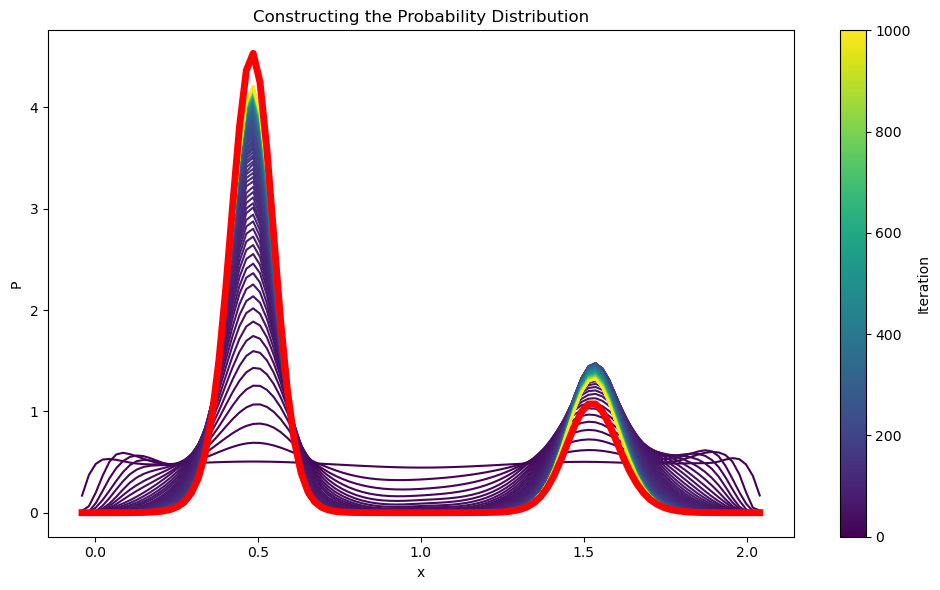
\includegraphics[width=0.51\textwidth]{images/two_well_wham.png} }}%
    \qquad
    \subfloat[\centering Free Energy Profile]{{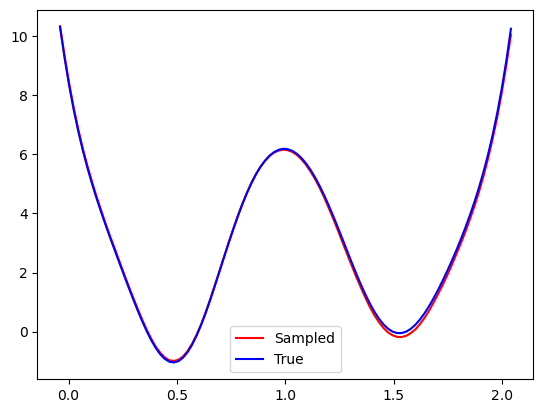
\includegraphics[width=0.41\textwidth]{images/two_well_free_energy.png} }}%
    \caption{Unbiased Densities and Free Energy Profile}%
    \label{fig:unbiased_densities}%
\end{figure}

In Figure \ref{fig:unbiased_densities}, we plot the global unbiased probabilities of $x$ for every iteration of WHAM. We can see that the probabilities converge to a stable distribution, which is the true distribution of $x$ in the system (the red curve), which is given by $P(x) \propto e^{-\beta V(x)}$. This indicates that WHAM has successfully unbiased the biased distributions. Similarly, we see that the computed free energy profile of the system as a function of $x$ is accurate.

\subsubsection{Comparison with Metroplis-Hastings}

We also compared the energy profile obtained from umbrella sampling and WHAM with the energy profile obtained from a standard Metropolis-Hastings simulation. We ran a Metropolis-Hastings simulation for 1,000,000 steps, and calculated the free energy profile of the system as a function of $x$.

\begin{figure}%
    \centering
    \subfloat[\centering Probability Distribution]{{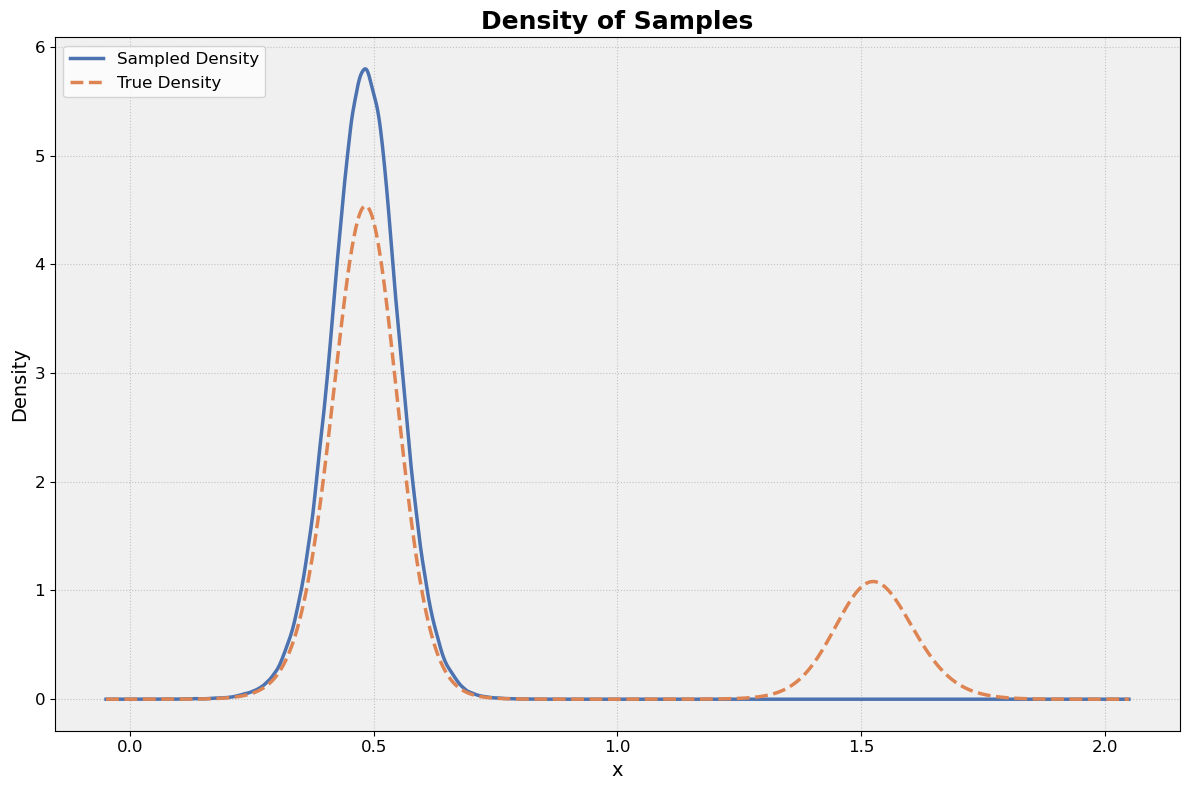
\includegraphics[width=0.46\textwidth]{images/metro_hastings_density.png} }}%
    \qquad
    \subfloat[\centering Free Energy Profile]{{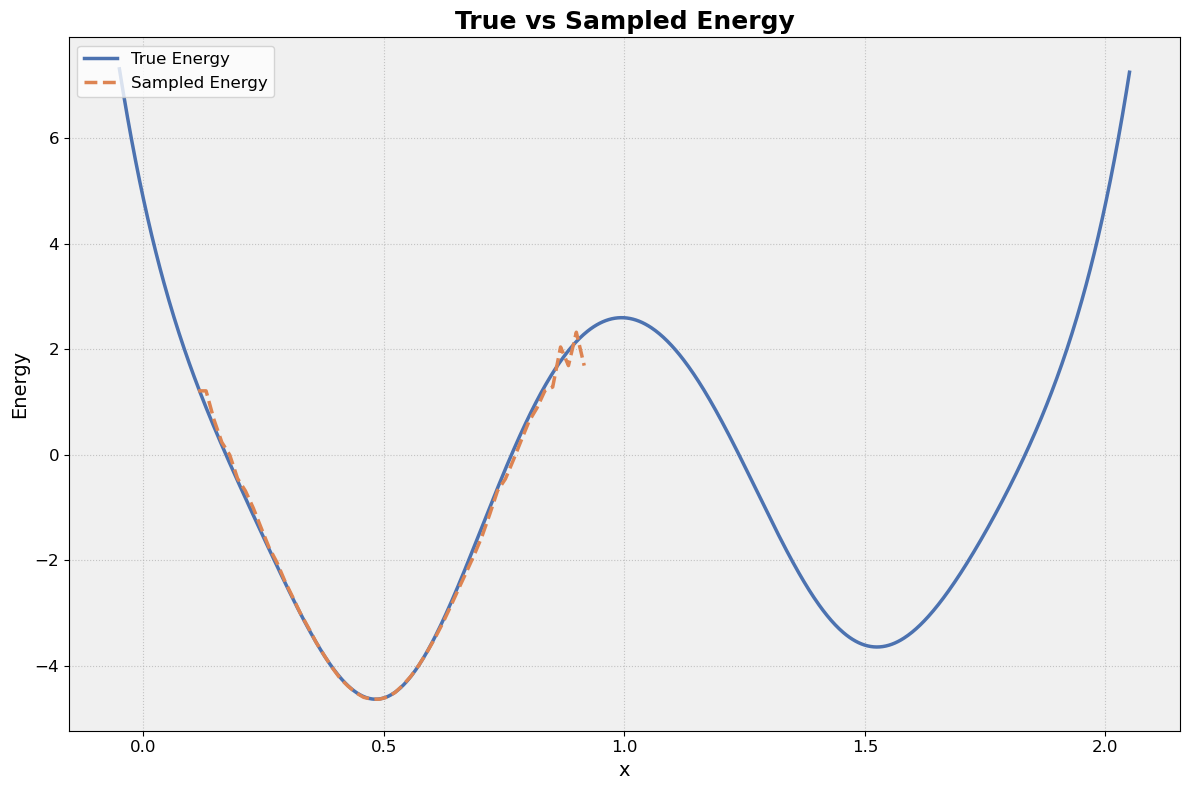
\includegraphics[width=0.46\textwidth]{images/metro_hastings_energy.png} }}%
    \caption{Unbiased Densities and Free Energy Profile}%
    \label{fig:metro_hastings_plot}%
\end{figure}

In Figure \ref{fig:metro_hastings_plot}, we plot the probability distribution of $x$ obtained from the Metropolis-Hastings simulation, and the potential energy profile of the system as a function of $x$. We can see that because of the high energy barrier in the potential, as well as the low temperature of the system, the standard Metropolis-Hastings simulation is unable to sample the potential energy surface effectively, and gets stuck in the local minima. This results in a free energy profile doesn't fully capture the entire domain of the system. In contrast, the free energy profile obtained from umbrella sampling and WHAM captures the entire domain of the system, and is able to accurately sample the potential energy surface.

\subsection{1D Multi-Welled Potential}

Similarly, we divided our one-dimensional multi-welled potential into 100 windows, each with a biasing potential of the same form as the two-welled potential. We then ran MCMC simulations in each window, obtaining $100,000$ samples for each window, resulting in biased distributions of $x$.

\end{document}
